\documentclass[letterpaper]{article}
\usepackage[margin=1in]{geometry} % Sets page size and 1-inch margins
\usepackage[svgnames,dvipsnames]{xcolor}   % For a wider range of colors

\usepackage{amsmath} % For math symbols like \lor, \langle, \rangle, \to
\usepackage{array}   % For advanced column specifications
\usepackage{tabularx}% For tables with auto-expanding columns
\usepackage{tikz}
\usetikzlibrary{
    positioning,      % For placing nodes relative to each other (e.g., below=of)
    shapes.geometric, % For shapes like ellipses
    arrows.meta,      % For advanced arrow tips (e.g., Stealth)
    decorations.pathmorphing, % For snake/squiggly lines
    calc              % For coordinate calculations
}

% --- GLOBAL STYLE DEFINITIONS FOR DFD ---
\tikzset{
    % A shape for logical connectives
    connective_node/.style={
        rectangle, rounded corners=5pt, draw=black!80, fill=black!10,
        inner sep=5pt, thick, align=center
    },
    % A shape for Introduction Rules
    intro_rule_node/.style={
        rectangle, rounded corners=5pt, draw=black!80, fill=Teal!20,
        inner sep=5pt, thick, align=center
    },
    % A shape for Elimination Rules
    elim_rule_node/.style={
        rectangle, rounded corners=5pt, draw=black!80, fill=BurntOrange!20,
        inner sep=5pt, thick, align=center
    },
    % A shape for abstract propositions
    proposition_node/.style={
        ellipse, draw=black!80, fill=Violet!15,
        inner sep=3pt, align=center
    },
    % A shape for concrete proof terms
    proof_node/.style={
        ellipse, draw=black!80, fill=Green!15,
        inner sep=3pt, align=center
    },
    % Interface ports for composition
    input_port/.style={
        circle, draw=blue!70!black, fill=blue!20,
        inner sep=2pt, minimum size=8pt
    },
    output_port/.style={
        circle, draw=ForestGreen!80!black, fill=ForestGreen!20,
        inner sep=2pt, minimum size=8pt
    },
    % Arrow styles with color
    input_arrow/.style={-Stealth, solid, thick, draw=blue!70!black},
    output_arrow/.style={double, double distance=1.5pt, -Stealth, solid, thick, draw=ForestGreen!80!black},
    proves_arrow/.style={-Stealth, decorate, decoration={snake, segment length=6pt, amplitude=1pt}, thick, draw=orange!90!black}
}

% --- Define and measure boxes to get widths for tabularx ---
\newlength{\orheaderwidth}
\settowidth{\orheaderwidth}{\textbf{Or} : Prop $\to$ Prop $\to$ Prop}
\addtolength{\orheaderwidth}{1em}

\begin{document}

\begin{figure}[h!]
\centering
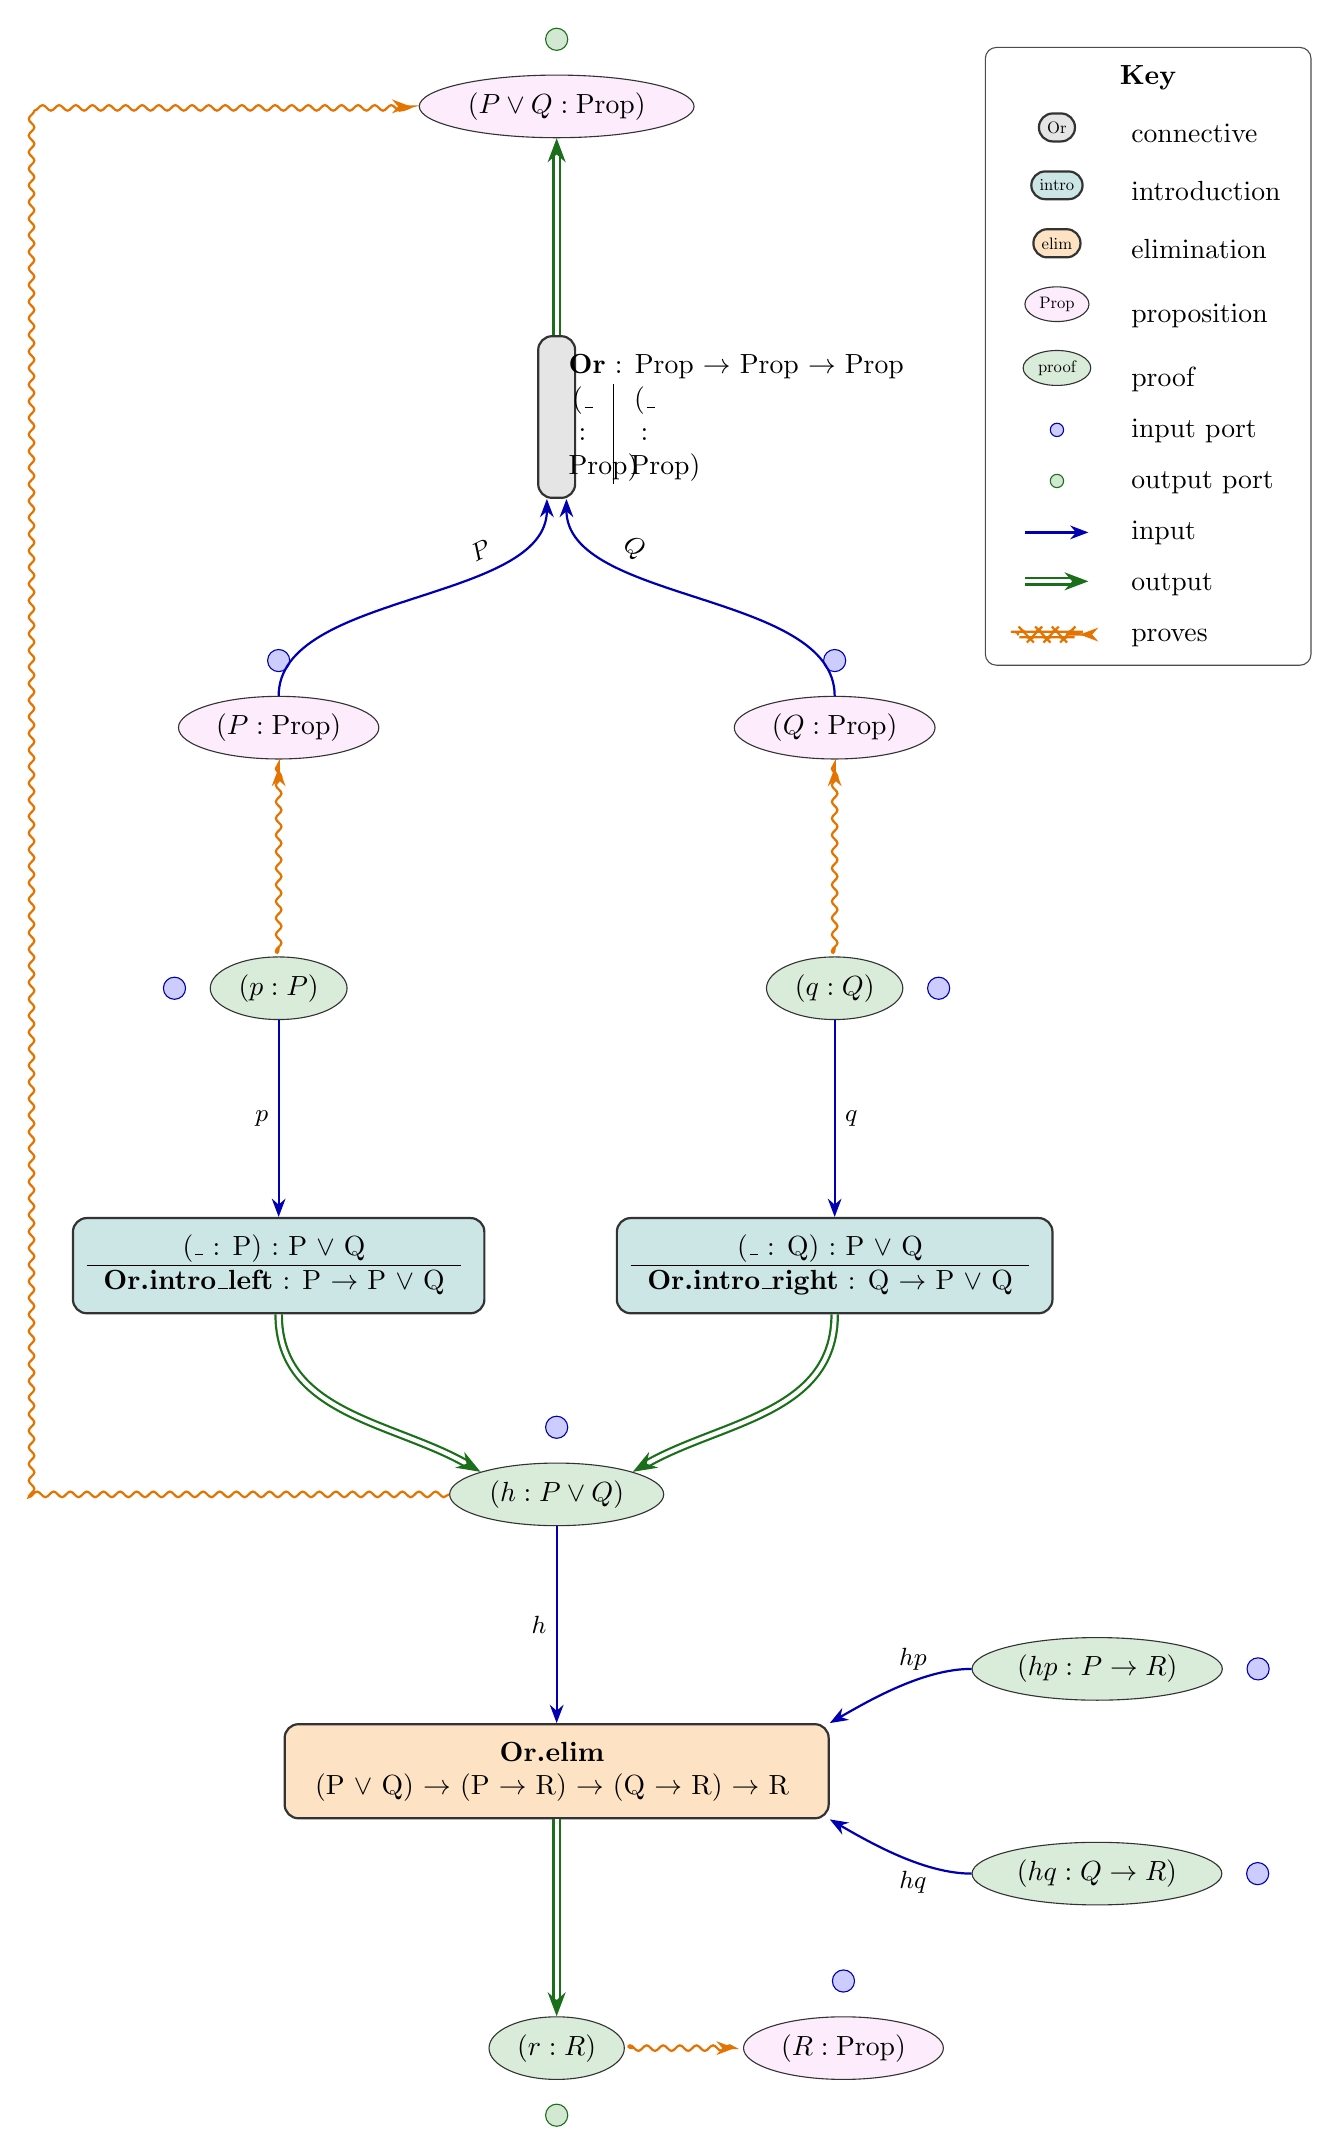
\begin{tikzpicture}[node distance=2.5cm and 2.5cm]

% --- INPUT TYPE PARAMETERS ---
\node[proposition_node] (P_prop) {$(P : \text{Prop})$};
\node[proposition_node] (Q_prop) [right=4.5cm of P_prop] {$(Q : \text{Prop})$};

% Input ports for type parameters
\node[input_port] (P_in_port) [above=0.3cm of P_prop] {};
\node[input_port] (Q_in_port) [above=0.3cm of Q_prop] {};

% --- CONNECTIVE LAYER ---
\node[connective_node, above=2.5cm of $(P_prop.north)!.5!(Q_prop.north)$] (or_box) {
    \begin{tabularx}{\orheaderwidth}{>{\centering\arraybackslash}X|>{\centering\arraybackslash}X}
        \multicolumn{2}{c}{\textbf{Or} : Prop $\to$ Prop $\to$ Prop} \\ \hline
        (\_ : Prop) & (\_ : Prop)
    \end{tabularx}
};

\node[proposition_node] (P_or_Q_prop) [above=2.5cm of or_box] {$(P \lor Q : \text{Prop})$};

% Output port for result type
\node[output_port] (type_out_port) [above=0.3cm of P_or_Q_prop] {};

% --- INTRODUCTION SECTION ---
\node[proof_node] (p_P) [below=2.5cm of P_prop] {$(p : P)$};
\node[proof_node] (q_Q) [below=2.5cm of Q_prop] {$(q : Q)$};

% Input ports for proof terms
\node[input_port] (p_in_port) [left=0.3cm of p_P] {};
\node[input_port] (q_in_port) [right=0.3cm of q_Q] {};

\node[intro_rule_node, below=2.5cm of p_P] (or_inl) {
    \begin{tabular}{c}
    (\_ : P) : P $\lor$ Q \\ \hline
    \textbf{Or.intro\_left} : P $\to$ P $\lor$ Q
    \end{tabular}
};

\node[intro_rule_node, below=2.5cm of q_Q] (or_inr) {
    \begin{tabular}{c}
    (\_ : Q) : P $\lor$ Q \\ \hline
    \textbf{Or.intro\_right} : Q $\to$ P $\lor$ Q
    \end{tabular}
};

% --- ELIMINATION SECTION ---
\node[proof_node] (h_P_or_Q) [below=2.5cm of $(or_inl)!.5!(or_inr)$] {$(h : P \lor Q)$};

% Input port for disjunction proof
\node[input_port] (h_in_port) [above=0.3cm of h_P_or_Q] {};

\node[elim_rule_node, below=2.5cm of h_P_or_Q] (or_elim) {
    \begin{tabular}{c}
    \textbf{Or.elim} \\
    (P $\lor$ Q) $\to$ (P $\to$ R) $\to$ (Q $\to$ R) $\to$ R
    \end{tabular}
};

% Case continuation proofs
\node[proof_node] (hp_P_to_R) [right=1.8cm of or_elim, yshift=1.3cm] {$(hp : P \to R)$};
\node[proof_node] (hq_Q_to_R) [right=1.8cm of or_elim, yshift=-1.3cm] {$(hq : Q \to R)$};

% Input ports for case continuations
\node[input_port] (hp_in_port) [right=0.3cm of hp_P_to_R] {};
\node[input_port] (hq_in_port) [right=0.3cm of hq_Q_to_R] {};

% Result and target type
\node[proof_node] (result_R) [below=2.5cm of or_elim] {$(r : R)$};
\node[proposition_node] (R_prop) [right=1.5cm of result_R] {$(R : \text{Prop})$};

% Input port for target type R
\node[input_port] (R_in_port) [above=0.3cm of R_prop] {};

% Output port for result
\node[output_port] (r_out_port) [below=0.3cm of result_R] {};

% --- EDGE ROUTING ---
\draw[output_arrow] (or_box) -> (P_or_Q_prop);
\draw[input_arrow] (P_prop.north) to[out=90, in=-90, looseness=0.8] node[pos=0.7, sloped, above, font=\small] {$P$} ($(or_box.south west)!.5!(or_box.south)$);
\draw[input_arrow] (Q_prop.north) to[out=90, in=-90, looseness=0.8] node[pos=0.7, sloped, above, font=\small] {$Q$} ($(or_box.south)!.5!(or_box.south east)$);

\draw[input_arrow] (p_P) -> node[left, font=\small] {$p$} (or_inl.north);
\draw[input_arrow] (q_Q) -> node[right, font=\small] {$q$} (or_inr.north);

\draw[output_arrow] (or_inl.south) to[out=-90, in=150] (h_P_or_Q.north west);
\draw[output_arrow] (or_inr.south) to[out=-90, in=30] (h_P_or_Q.north east);

\draw[input_arrow] (h_P_or_Q) -> node[left, font=\small] {$h$} (or_elim);
\draw[input_arrow] (hp_P_to_R) to[out=180, in=30, looseness=0.8] node[pos=0.4, above, font=\small] {$hp$} (or_elim.north east);
\draw[input_arrow] (hq_Q_to_R) to[out=180, in=-30, looseness=0.8] node[pos=0.4, below, font=\small] {$hq$} (or_elim.south east);
\draw[output_arrow] (or_elim) -> (result_R);

% Proves arrows
\draw[proves_arrow, shorten <=3pt, shorten >=3pt] (p_P) -> (P_prop);
\draw[proves_arrow, shorten <=3pt, shorten >=3pt] (q_Q) -> (Q_prop);
\draw[proves_arrow, shorten <=3pt, shorten >=3pt] (result_R) to[out=0, in=180] (R_prop);

% Main "proves" arc
\coordinate (outset_point) at ($(P_prop.west)+(-1.8cm,0)$);
\draw[proves_arrow, shorten >=3pt] (h_P_or_Q.west) -- (outset_point |- h_P_or_Q.west) -- (outset_point |- P_or_Q_prop.west) -- (P_or_Q_prop.west);

% --- LEGEND ---
\node (legend) [draw=black!70, rounded corners, inner sep=5pt, above right=0.5cm and 1cm of Q_prop] {
    \begin{tabular}{cl}
    \multicolumn{2}{c}{\textbf{Key}} \\[1.5ex]
    \tikz{\node[connective_node, scale=0.6] {Or};} & connective \\[1.5ex]
    \tikz{\node[intro_rule_node, scale=0.6] {intro};} & introduction \\[1.5ex]
    \tikz{\node[elim_rule_node, scale=0.6] {elim};} & elimination \\[1.5ex]
    \tikz{\node[proposition_node, scale=0.6] {Prop};} & proposition \\[1.5ex]
    \tikz{\node[proof_node, scale=0.6] {proof};} & proof \\[1.5ex]
    \tikz{\node[input_port, scale=0.6] {};} & input port \\[1.5ex]
    \tikz{\node[output_port, scale=0.6] {};} & output port \\[1.5ex]
    \tikz{\draw[input_arrow] (0,0.1) -- (0.8,0.1);} & input \\[1.5ex]
    \tikz{\draw[output_arrow] (0,0.1) -- (0.8,0.1);} & output \\[1.5ex]
    \tikz{\draw[proves_arrow] (0,0.1) -- (0.8,0.1);} & proves \\
    \end{tabular}
};

\end{tikzpicture}
\caption{Modular Or connective with composition interfaces. Input ports accept type parameters and proof terms. The dual introduction rules inject into the sum type, while elimination requires case analysis with continuation functions. Output ports provide results for composition.}
\label{fig:or_modular}
\end{figure}

\end{document}